% A 2-colouring of the subsets of {1,2,3}, drawn on the cube.
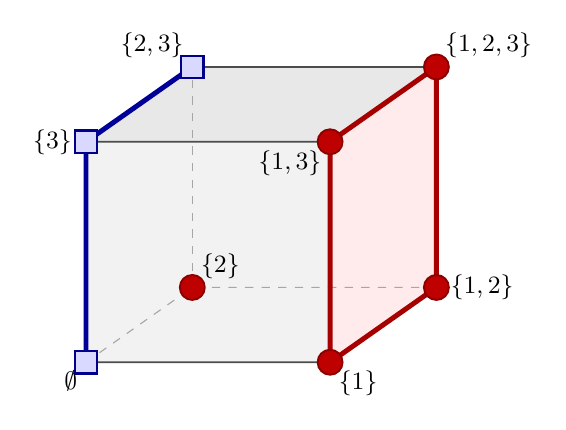
\begin{tikzpicture}[
    x={(3.1cm,0cm)}, y={(1.35cm,0.95cm)}, z={(0cm,2.8cm)},
    red/.style={circle, draw=red!55!black, fill=red!75!black, line width=0.7pt,
      inner sep=0pt, minimum size=9pt},
    blue/.style={rectangle, draw=blue!55!black, fill=blue!15, line width=0.9pt,
      inner sep=0pt, minimum size=8pt},
    lab/.style={font=\small, inner sep=2pt}]
  % faces
  \fill[gray!10] (0,0,0) -- (1,0,0) -- (1,0,1) -- (0,0,1) -- cycle;
  \fill[gray!18] (0,0,1) -- (1,0,1) -- (1,1,1) -- (0,1,1) -- cycle;
  \fill[red!8]   (1,0,0) -- (1,1,0) -- (1,1,1) -- (1,0,1) -- cycle;
  % hidden edges
  \draw[dashed, gray!70] (0,0,0) -- (0,1,0) -- (1,1,0);
  \draw[dashed, gray!70] (0,1,0) -- (0,1,1);
  % visible edges
  \draw[gray!60!black, line width=0.6pt]
    (0,0,0) -- (1,0,0) -- (1,1,0) -- (1,1,1) -- (0,1,1) -- (0,0,1) -- cycle
    (1,0,0) -- (1,0,1) -- (1,1,1)
    (0,0,1) -- (1,0,1);
  % the red family: the red face together with {2}
  \draw[red!65!black, line width=1.8pt]
    (1,0,0) -- (1,1,0) -- (1,1,1) -- (1,0,1) -- cycle;
  % the blue chain
  \draw[blue!60!black, line width=1.8pt] (0,0,0) -- (0,0,1) -- (0,1,1);
  % vertices
  \node[blue] (e)   at (0,0,0) {};
  \node[red]  (a)   at (1,0,0) {};
  \node[red]  (b)   at (0,1,0) {};
  \node[blue] (c)   at (0,0,1) {};
  \node[red]  (ab)  at (1,1,0) {};
  \node[red]  (ac)  at (1,0,1) {};
  \node[blue] (bc)  at (0,1,1) {};
  \node[red]  (abc) at (1,1,1) {};
  \node[lab, below left=1pt]            at (e)   {$\emptyset$};
  \node[lab, below right=1pt]           at (a)   {$\{1\}$};
  \node[lab, above right=1pt]           at (b)   {$\{2\}$};
  \node[lab, left=3pt]                  at (c)   {$\{3\}$};
  \node[lab, right=3pt]                 at (ab)  {$\{1,2\}$};
  \node[lab, below left=1pt]            at (ac)  {$\{1,3\}$};
  \node[lab, above left=1pt]            at (bc)  {$\{2,3\}$};
  \node[lab, above right=1pt]           at (abc) {$\{1,2,3\}$};
\end{tikzpicture}
